\section{Study Application}
This section will describe the study application in terms of components and will illustrate how the application looked.

\subsection{Installing the Application}
The application was only released on iOS as previously mentioned and therefore was distributed exclusively via the Apple App Store. When beta testing iOS applications one can use the TestFlight service provided by Apple which essentially functions a separate App Store for applications in development, which require an invitation to install. Once the user had such an invitation the installation process was the following: The user installs the TestFlight application via the App Store, then opens the TestFlight application to find the Mobility Study app ready for installation. Once the Mobility Study app is installed, it will ask for permission to track the user's location as well as sending the user notifications. The location tracking is obviously necessary for the collection of location data, the notifications are not necessary but help the user be reminded to fill out a daily questionnaire. An installation manual (see Appendix \ref{appendix:installation} was provided to the participants to ensure the applications were set up correctly. The installation process is shown in Figure \ref{fig:screens-install}.

\begin{figure}
    \centering
    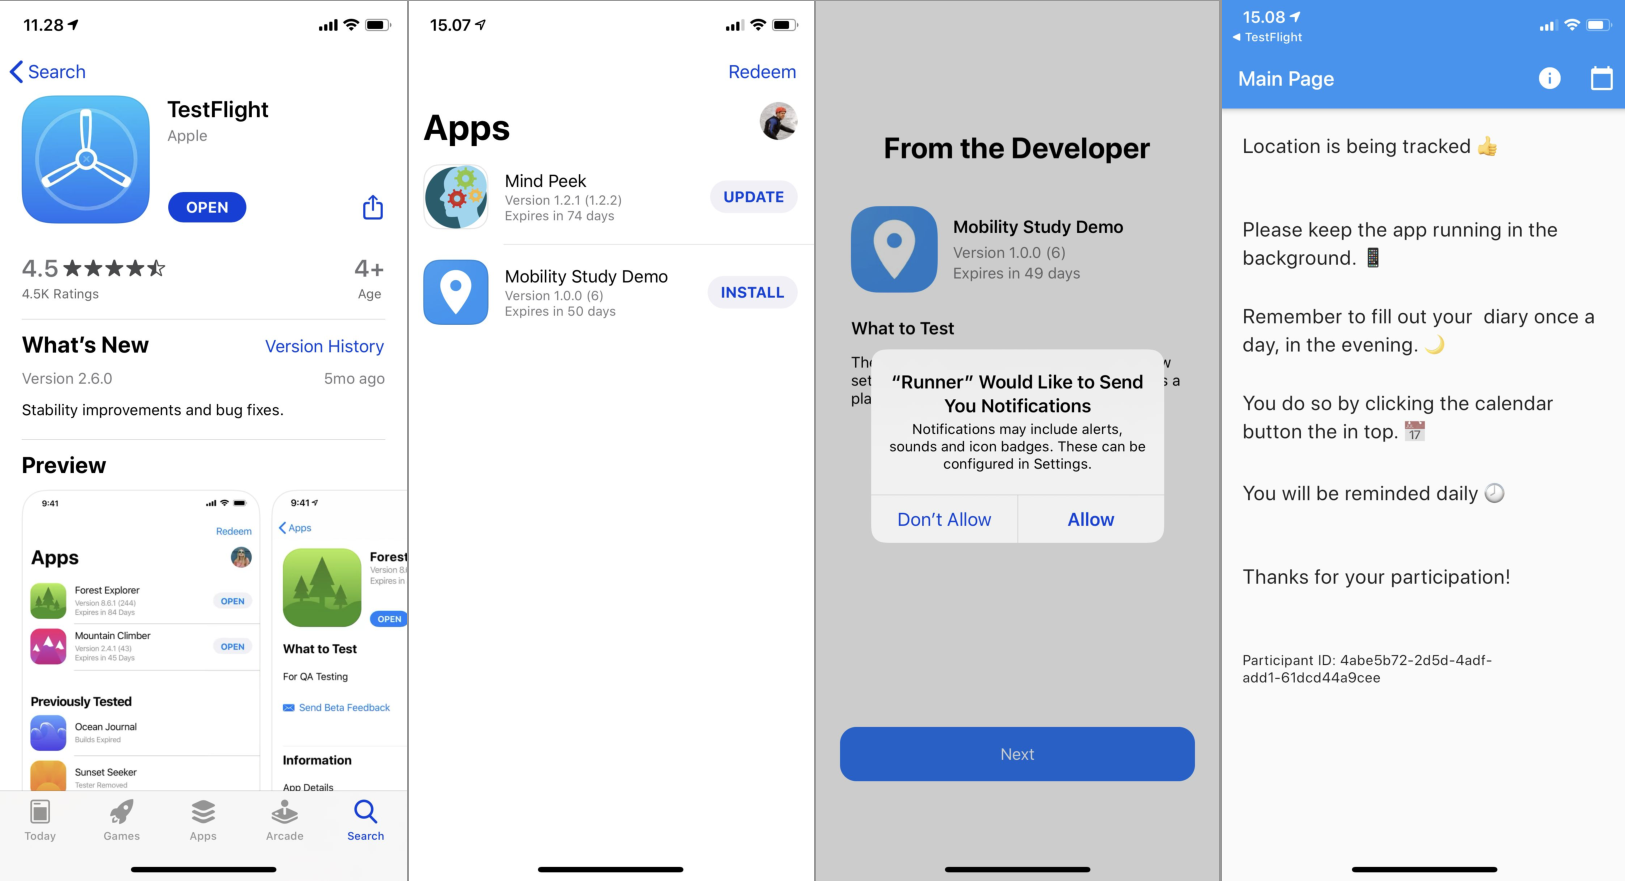
\includegraphics[width=\textwidth]{images/app_imgs/screens-install.pdf}
    \caption{The initial installation- and setup process for the user}
    \label{fig:screens-install}
\end{figure}

\subsection{App Screens}
The Main Page of the application merely displays a list of instructions to the user but has two buttons in the navigation bar which can take the user to the Info Page and the Diary Page. The Info Page is made to inform the user of how the data will be used, and an email to contact the researcher in case of any questions. The user navigates to the Diary Page by either tapping the calendar icon on the main page or by tapping the notification which comes in daily. In total there are four answers which answer answered by pressing the Answer button; this shows a wheel of possible values to pick from for providing an answer. Once all answers have been given, the submit button will be enabled, and once pressed the answers will be stored on the device and sent to a server. When this is done, the last screen will appear which informs the user the answers have been saved and thanks them for their contribution.

\begin{figure}
    \centering
    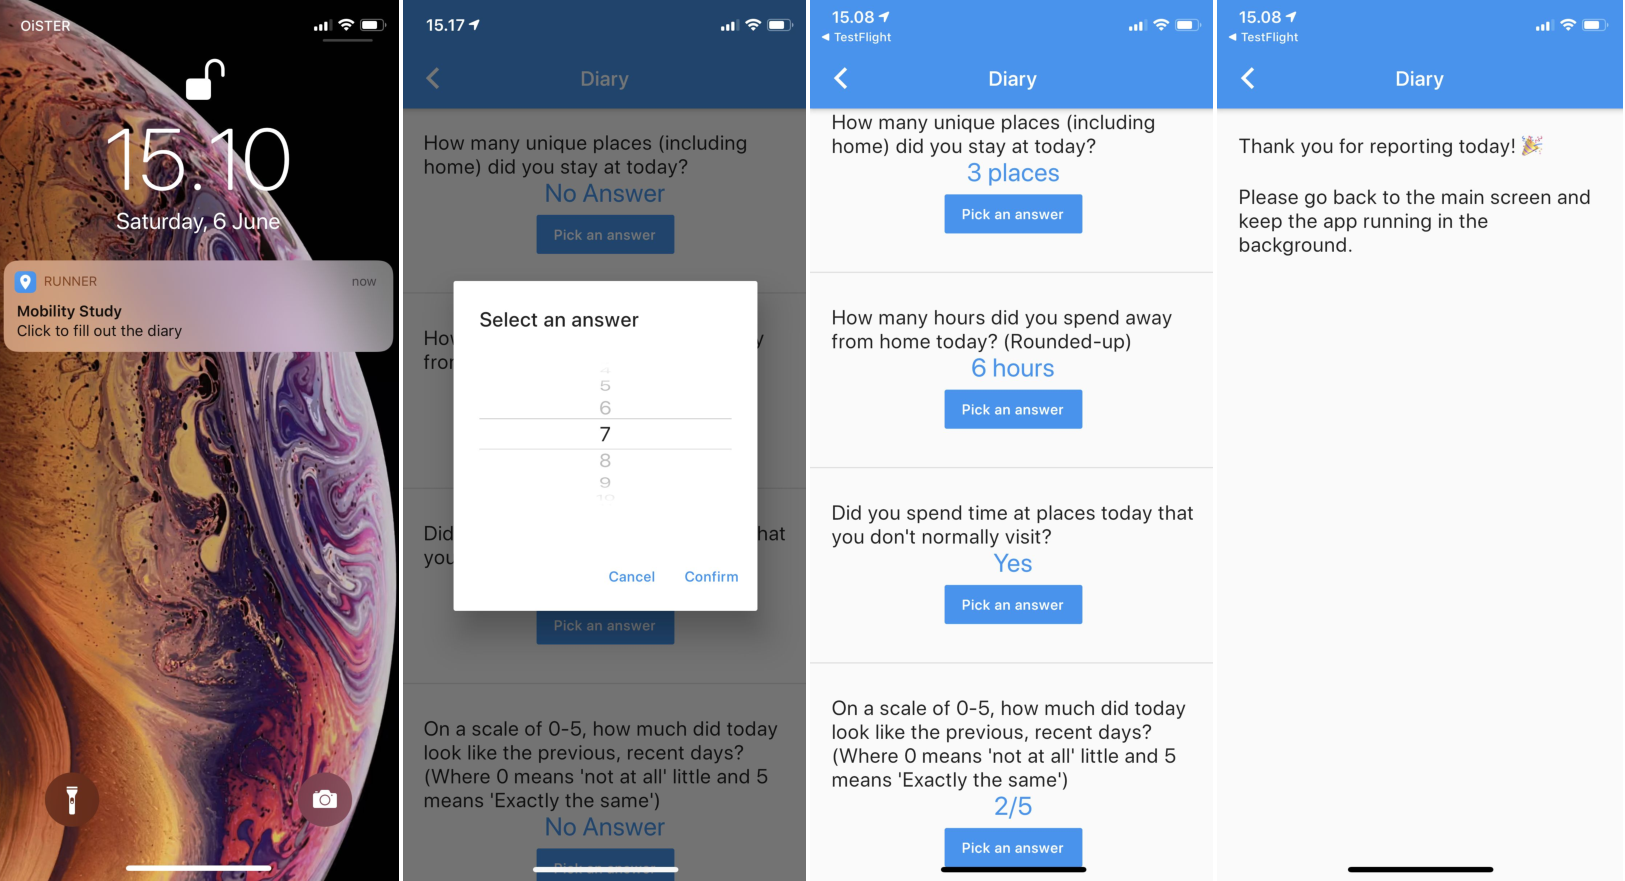
\includegraphics[width=\textwidth]{images/app_imgs/screens-answers.pdf}
    \caption{The different screens which the user is taken through for submitting answers}
    \label{fig:screens-answers}
\end{figure}

\subsection{Displaying Features}
An initial version of the application included a display of the real-time calculated features, which were recalculated each time a button was pressed. It was decided to not display the features in the final version for the study since they would influence the answers given by the users. For example, if the application would state that the user has visited a certain number of places today, it is highly unlikely that a participant would report something else if they are the least in doubt themselves. This display of features may be relevant (at least for some of the more features which are more easily interpret-able such as Home Stay) for a real-world application where it makes sense to inform the user exactly what goes on behind the curtain.

\begin{figure}
    \centering
    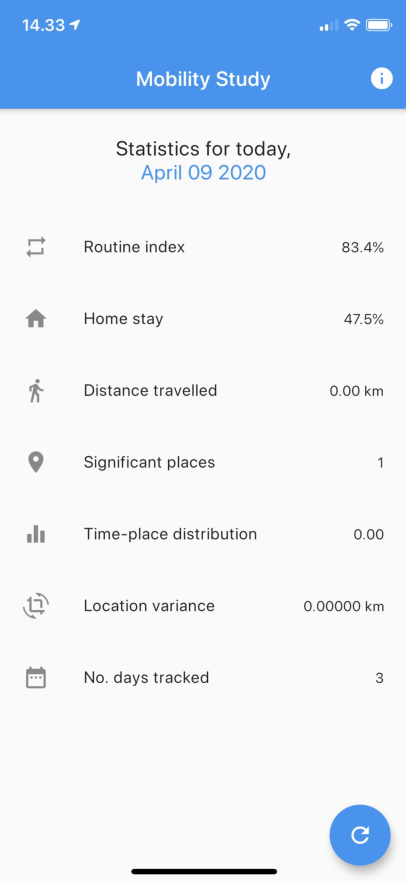
\includegraphics[width=0.3\textwidth]{images/app_imgs/screens-features.pdf}
    \caption{An early iteration of the study app in which the feature values were shown}
    \label{fig:app-features-screen}
\end{figure}
\subsection{Data Storage}
To store the data from the study online, such that it could later be extracted for data analysis, a Firebase file storage server was used for uploading files multiple times daily. Concretely, the LocationSamples, Stops, and Moves were stored locally on the device. Whenever a Feature calculation was triggered, the calculated MobilityContext was serialized and uploaded as a file, in addition to the data points for the day and all Stops and Moves on the phone for the period. This process was very wasteful in the sense that only 'new' data points needed to be uploaded, but instead, the whole file was just overwritten. This was mainly done to ensure little data loss and avoid inconsistencies between the online file and the local file.